% !TeX spellcheck = da_DK
\section{Systembeskrivelse} \fxnote{Erika har tegnet en ring om "med et accelerometer" i problemanalysen} 
Dette afsnit indeholder en beskrivelse af det system, der skal kunne anvendes af apopleksipatienter som et selvstændigt træningsapparat i rehabiliteringen af balanceproblemer. Systembeskrivelsen indeholder målgruppen for designet, samt hvilket formål og anvendelse det har. Ud fra disse faktorer er systemet blevet designet og illustreret i et blokdiagram. 

\subsection{Systemets bruger}
Systemet udvikles til apopleksipatienter med balanceproblemer mhp. selvtræning af balance i rehabiliteringsfasen, der bliver omtalt som fase 3 og 4 i afsnit \ref{Faser} på side \pageref{Faser}. Jævnfør afsnit \ref{Indledning} på side \pageref{Indledning} ses det, at majoriteten af apopleksipatienter er over 65 år, og systemet skal derfor være let anvendeligt. Systemets design skal altså være enkelt, så der ikke skabes forvirring blandt brugerne ift. systemets funktioner. Fagkyndigt personale, såsom fysioterapeuter og læger, skal kunne instruere patienten i brugen af systemet samt følge med i udviklingen, som patienten gennemgår. Det skal derfor være muligt for det fagkyndige personale at anvende systemet og aflæse data herfra. Dette gøres ved, at systemet både har et analogt og digitalt output, hvor den digitale del henvender sig til det fagkyndige personale i form af grafer, mens den analoge del henvender sig til apopleksipatienterne. \fxnote{Erikas kommentar: relevans ift. analogt og digitalt output? Tekniske detaljer! Er det vigtigt, at det er et analog output eller at det output indeholder specifik information?}   

\subsection{Systemets formål og anvendelse}
Systemets input er patienternes kropshældning, dvs. hvor meget vedkommende svajer i anatomisk position og under udførelse af en bestemt øvelse. Systemet skal kunne konvertere informationerne vedrørende patienternes kropshældning til visuel og sensorisk feedback, samt et digitalt output i form af grafer. Den visuelle og sensoriske feedback har til formål at gøre apopleksipatienter opmærksomme på, hvornår de har bevæget sig over den normale grænse for krops svaj. Således kan systemet registrere, hvis patienten er i risiko for at falde. Inden et fald sker udsendes et feedback signal, så patienterne har mulighed for at rette sig op. Selve systemet skal anvendes til selvtræning i hjemmet. Det skal derfor være et brugervenligt system, dvs. systemet skal kunne påsættes uden problemer og fungere uden, at patienten skal navigere rundt i forskellige funktioner for at påbegynde feedbacken. Systemet skal fungere som en hjælp for patienten, da vedkommende bliver bevidst omkring sin balance. Herved kan patienten være mere selvstændig i rehabiliteringsprocessen.

Systemet designes til selvtræning af statisk balance. Patienterne kan anvende systemet ved to sværhedsgrader: Ved normal kropsstilling (anatomisk udgangsposition) og en bestemt øvelse, som patienterne skal udføre. Apopleksipatienternes balance udfordres i højere grad af øvelsen end ved normal kropsstilling, eftersom kropsvægten fordeles anderledes ved øvelsen ift. den normale kropsstilling omtalt i afsnit \ref{BalanceAfsnit} på side \pageref{BalanceAfsnit}. Øvelsen foretages i stående udgangsposition med fødderne på en tegnet linje, så den ene fods tæer er mod den anden fods hæl. %Denne position er valgt for at udfordre patientens balance ved at fordele kropsvægten anderledes ift. den normale kropsstilling omtalt i afsnit \ref{BalanceAfsnit} på side \pageref{BalanceAfsnit}. % Patienten påsætter selv systemet øverst på sternum og udfører herefter en kort prøvetest for at kende til de givne feedback parametre.Under prøvetesten svajer patienten langsomt fra side til side. 
%Det er på baggrund af afsnit \ref{MekBioFeed} på side \pageref{MekBioFeed} valgt at hældningen på patienten skal opfanges vha. et accelerometer, der er placeret øverst på sternum. 
Det er på baggrund af afsnit \ref{MekBioFeed} på side \pageref{MekBioFeed} valgt, at systemet skal placeres øverst på sternum for at få bedst mulige målinger ift. patienternes kropshældning. Systemet skal give sensorisk og visuel feedback i form af en vibrator samt fem dioder bestående af en grøn, to gule og to røde. Som udgangspunkt svajer kroppens position omkring seks til syv grader i lateral retning \cite{Wang2010} \fxnote{Vi skal have noget point of no return ind her ift fald}, så hvis patienternes kropshældning ligger over denne værdi er de i fare for at miste balancen. Hvis patienten hælder i intervallet $8^{\circ}$-$13^{\circ}$ til højre, indikeres dette af den gule diode på højresiden af den grønne diode. Derudover aktiveres en mild vibration, når den gule diode lyser. Hvis patienten hælder $13^{\circ}$ eller derover, lyser den røde diode til højre for den gule diode og styrken af vibrationen forøges. Det samme gør sig gældende for hældning mod venstre. Med denne metode indikeres både, hvilken retning patienten svajer samt graden heraf. Ved benyttelse af to feedback former er der større mulighed for, at patienten kan opfange signalerne. Hvis patientens visuelle sans er begrænset kan systemet stadig benyttes grundet den sensoriske feedback. \\ 
Efter en testøvelse af systemet udføres selve træningsøvelsen, hvor udgangspositionen indtages på linjen. For at øge sværhedsgraden yderligere kan den visuelle sans udelukkes. Patienten skal under øvelsen forsøge at holde balancen så længe som muligt uden at bevæge sig ud i risikozonerne. Hvis patienten kommer ud i risikozonerne vil dette blive markeret ved lys i dioderne samt vibration. Træningsøvelsen gentages efter behov. Ved at tage flere målinger igennem rehabiliteringsforløbet vil det forventes, at der sker en fremgang ift. tiden, hvori balancen kan opretholdes uden at patienten bevæger sig ud i risikozonerne. 

%\subsection{Accelerometer}
%I forsøget anvendes ADXL327 som er et tre-akset accelerometer ift. forsøget gives det elektriske signal ud fra X og Z-aksen. Produktet måler accelerationen med minimum fuldskala på \pm 2g. Sensitiviteten afhænger af forsyningsspændingen og ved 3V er sentivitivten 420mv/g. 

%Ledningerne snoes for at kontrollere samt mindske støjen. Derudover sættes ledninger fast med tape på patienten, så vidt det er muligt. For at undgå unødvendigt støj foretages forsøget væk fra andet elektronik.  %\ref{reference til støj afsnittet}

%\subsection{Analogt output}
%Det analoge output skal kunne henvende sig til patienten, dette sker ved lysdioder og vibration. Lysdioderne skal lyse gult ved 'usikkerhed' og slukke hvis patienten enten er rettet op igen eller bevæger sig ud i riskozonen, hvorefter en ny diode skal lyse rødt. Vibrationerne igangsættes ved 'usikkerhed' og skal stoppe hvis patienten retter sig op eller stige i styrke, hvis patienten kommer ud i risikozonen. 

%\subsection{Digitalt output}
%Det digitale skal kunne anvendes af sundhedspersonale til at vurdere om patienten gør fremskridt, dette indebærer at informationerne for patienten kan gemmes og sammenlignes på en computer. 


\subsection{Systemets opbygning} \fxnote{Ny figur - Erika: strømforsyning?}
Systemets opbygning fremgår af \figref{kravblok}.

\begin{figure}[H]
	\centering
	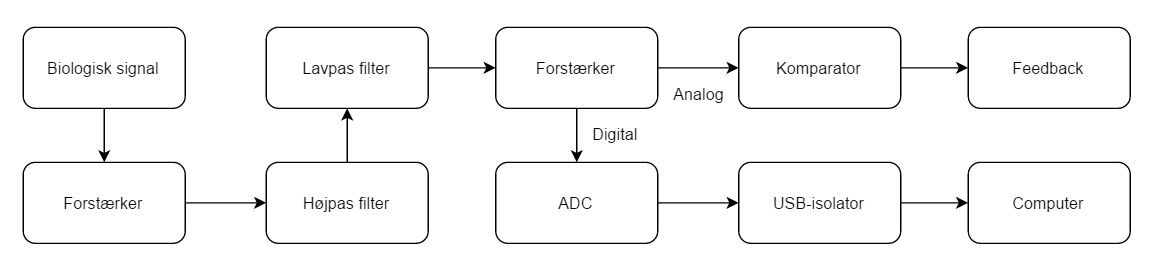
\includegraphics[scale=0.7]{figures/cProblemloesning/Systemopbygning.PNG}
	\caption{Figuren viser de enkelte blokke, som systemet skal indeholde.}
	\label{kravblok}
\end{figure}

%Det biologiske signal der opnås fra accelrometeret skal forstærkes (instrumenteringsforstærker?). Dette gøres fordi signalerne der opfanges er meget små og det vil derfor gøre filtreringen mere præcis ved at forstærke signalet.
%Herefter benyttes der et højpas filter for at frasortere den støj der kommer fra tyngdekraften. \fxnote{Der skal tilføjes noget om højpas filter ligesom det der står ved lavpas filter} 
Det biologiske signal der opnås fra accelerometeret skal som det første filtreres vha. et lavpasfilter. Dette gøres for at frasortere uønskede frekvenser  over 45 Hz. Grunden til disse frekvenser kan frasorteres, er at det signal som skal måles ligger under 45 Hz. Efter filtreringen af signalet benyttes en variabel forstærker, for at tilpasse signalets amplitude til ADC’en og komparatoren. Signalet ledes herefter videre i et analogt og digitalt kredsløb. I det analoge kredsløb kommer signalet først gennem en komparator. Denne skal sammenligne signalet der optages, så den rigtige feedback kan gives til patienten. Feedbacken bliver givet til patienten, således det bliver muligt at holde balancen, dette gøres i form at dioder og vibratorer. I det digitale kredsløb, bliver signalet ledt ind i en ADC. Denne vil omdanne det analoge biologiske signal til et digitalt signal. Det digitale signal bliver herefter ledt ind i en USB-isolator, så der ikke opstår lækstrømme og for at sikre patientens sikkerhed. Til sidst vil det digitale signal overført til en computer, hvor signalet herefter vil kunne gemmes. Det bliver herved muligt at databehandle signalet og opstille det som en graf eller lignende.

\subsection{Kravspecifikationer}
For at gøre anvendelse af samme system muligt til 4. Semester skal arbejdsområdet kunne benyttes sammen med et USB-baseret trådløst udviklingsværktøj eZ430-RF2500 fra Texas Instruments. Det er derfor nødvendigt, at designet stemmer overens med udviklingsværktøjet for at kunne sende og modtage data til og fra computeren. Udviklingsværktøjet indeholder hardware og software som evaluerer mikrokontrolleren MSP430F2274. For at hele vores system kan anvendes med udviklingsværktøjet, skal outputsignalet være 0-3V, eftersom mikrokontrolleren opererer med spændingsforsyning mellem 1,8V og 3,6V. \\
I praksis er det ikke muligt at have ideelle komponenter \fxnote{husk kilde}. Der vurderes derfor ud fra et pilotforsøg den tolerance, der accepteres ift. de enkelte blokke i systemet. Dette er udført mhp. at kunne beregne forstærkning, filtrering og integrering af signalet.\fxnote{Husk at opdatere her, når der kommer flere blokke}

\subsubsection{Det samlede system}
Systemet skal ved sammenligning af inputtet fra et flerakset accelerometeret og output fra dioder samt vibration give et analogt output. På denne måde vil aktivering af bestemte dioder og vibratorer afspejle inputsignalet, således at et input svarede til 8$^{\circ}$ aktiverer en gul diode og vibration, mens et input svarende til 13$^{\circ}$ vil aktivere en rød diode og stigningen i vibration. Derimod vil et input hvor opretholdelsen af balancen er korrekt svare til < 8$^{\circ}$, hvilket gør at den grønne diode vil lyse. Derudover vil det kunne bestemmes, hvilken retning patienten falder mod pga. accelerometerets 3 output akser, der kan måle i negativ og positiv retning. 

\textbf{Overordnede funktionelle krav til systemet:}
\begin{itemize}
\item Systemet skal være brugervenligt, så det kan anvendes af apopleksipatienter og fagkyndigt personale
\item Systemet skal kunne måle en apopleksipatients kropshældning, samt angive hvilken retning patienten hælder mod. Derudover skal det kunne måle statisk acceleration, eftersom vi måler på stående position.
\item Systemet skal kunne give visuel og sensorisk feedback til patienten ved forskellig hældningsgrad.
\item Grøn diode: Skal lyse, når patienten ikke er ude i risikozonerne.  
\item Gul diode: Skal lyse, når patienten hælder 8$^{\circ}$ og slukke, hvis patienten retter sig op eller hælder yderligere.
\item Rød diode: Skal lyse, når patienten hælder 13$^{\circ}$ eller mere og slukke, hvis patienten retter sig op.
\item Vibration: Skal aktiveres, hvis patienten hælder 8$^{\circ}$ og skal slukke, hvis patienten retter sig op. Hvis patienten hælder yderligere, skal vibrationshastigheden stige.
\item Systemet skal kunne skifte mellem to sværhedsgrader \fxnote{Hvordan skal hældningen i grader være ift. de to sværhedsgrader - skulle dioderne lyse ved forskellige grader}.
\item Signalet i systemet må ikke forstærkes til en værdi over 3V, da det så vil nå mætning.
\item Systemet skal kunne give et digitalt outout, så det er muligt at behandle og gemme patienternes data i et program.
\end{itemize}



%\textbf{Tolerance:}
%\begin{itemize}
%\end{itemize}
%
%\subsubsection{Accelerometer}
%\textbf{Krav:}
%\begin{itemize}
%\end{itemize}
%
%\textbf{Tolerance:}
%\begin{itemize}
%end{itemize}
%
%\subsubsection{Instrumentering forstærker}
%\textbf{Krav:}
%\begin{itemize}
%\end{itemize}
%
%\textbf{Tolerance:}
%\begin{itemize}
%\end{itemize}
%
%\subsubsection{Filtre - opdeling i høj og lavpass?}
%\textbf{Krav:}
%\begin{itemize}
%\end{itemize}
%
%\textbf{Tolerance:}
%\begin{itemize}
%\end{itemize}

%\subsubsection{Forstærker med variabel forstærkning}

%\textbf{Krav:}
%\begin{itemize}
%\end{itemize}
%
%\textbf{Tolerance:}
%\begin{itemize}
%\end{itemize}
%
%\subsubsection{Ensretter}

%\textbf{Krav:}
%\begin{itemize}
%\end{itemize}
%
%\textbf{Tolerance:}
%begin{itemize}
%end{itemize}
%
%\subsubsection{Integrator}
%\textbf{Krav:}
%\begin{itemize}
%\end{itemize}
%
%\textbf{Tolerance:}
%\begin{itemize}
%\end{itemize}
%
%\subsubsection{Advarsel}
%\textbf{Krav:}
%\begin{itemize}
%\end{itemize}
%
%\textbf{Tolerance:}
%\begin{itemize}
%\end{itemize}
%
%\subsubsection{ADC}
%Der anvendes en ADC i systemet, for at konvertere det analoge signal til digitalt. Den skal kunne sample det forstærkede signal. ADCens inputssignal vil ligge fra 0 til 3V. Det anbefales, at en ADC der skal opsamle et signal fra en variabel forstærkning har en opløsning på 12-bit \cite{Zouridakis2003}.
%\textbf{Krav:}
%\begin{itemize}
%\item Skal kunne modtage et inputssignal i intervallet 0 til 3 V.
%\item Skal have en samplingsfrekvens på minimum 100 Hz. 
%\end{itemize}

%\textbf{Tolerance:}
%\begin{itemize}
%\item Der accepteres ingen afvigelse ift. ADCen.
%\end{itemize}

%\subsubsection{USB-isolator}
%Systemet skal være sikkert for patienten at benytte, hvilket USB-isolatoren har til formål at sikre.
%\textbf{Krav:}
%\begin{itemize}
%\ Skal have den samme outputspænding som inputspænding. 
%\end{itemize}

%\textbf{Tolerance:}
%\begin{itemize}
%\item Der accepteres ingen afvigelse ift. USB-isolatoren. 
%\end{itemize}

%\subsubsection{Computer}
%Computeren er systemets digitale out. Det er brugerfladen for det fagkyndige personale og skal derfor kunne fremvise information omkring patienternes balance i form af grafer. Det fagkyndige personale skal vha. af programmet kunne følge med i patienternes udvikling ift. balancen og programmet hvori graferne vises skal derfor have følgende krav.
%\textbf{Krav:}
%\begin{itemize}
%\item Skal kunne fremvise en graf med information om patientens hældning i de enkelte øvelser. Herunder i hvor høj grad patienten har bevæget sig ud i risikozonerne. 
%\item Skal kunne gemme data, så fagkyndigt personale kan følge med i patienternes udvikling ift. balancen.
%\item Skal være brugervenligt for det fagkyndige personale, dvs. designet af programmet skal være enkelt. 
%\end{itemize}

%\textbf{Tolerance:}
%\begin{itemize}
%\item Der accepteres ingen afvigelse ift. computeren og det program det fagkyndige personale skal anvende. 
%\end{itemize}

%\item Systemet skal ved fald få dioder til at lyse samt give feedback i form af stigende vibration. 
%\item Systemet skal være non-invasiv - dvs. systemet ikke må påføre patienten smerte eller varig skade
%\item Systemet skal være brugervenligt
%\item Systemet skal forsynes med spænding fra 9V batteri
%\end{itemize}

%\subsubsection{Accelerometer}
%Accelerometeret skal detektere patientens kropshældning.

%\subsubsection{Filter}
%Når der anvendes et filter, skal det dæmpe uønskede frekvenser. Dvs. frekvenser der lavere eller højere ift. det signal fra accelerometeret, som man vil analysere på. Der skal udføres et pilotforsøg for at finde frem til det korrekte filter og valg af knækfrekvens. 

%\subsubsection{Signalerende lys}
%Når patienten er ude af balance skal en rød diode lyse, som signalering ift. patientens hældning. Der skal vha. et pilotforsøg detekteres, hvornår dioden skal lyse. Skal der evt. være 2 dioder, hvor den ene er et "advarende" signal og nr. to er "fare". 

%\subsubsection{Alarm/vibrationen}
%Alarmen/vibrationen skal anvendes i perioden, hvor patienten er ude af balance og stoppe igen, når der igen er oprettet balance. 
%(eller fungere som en alarm til dioderne - så når en diode lyser, skal alarmen gå)

%\subsubsection{ADC}
%Der anvendes en ADC i systemet, for at konvertere det analoge signal til digitalt. Det næste skridt er konverteringen til PC og det er derfor essentielt at have en ADC, der konverterer analogt signal til binære tal, som digitale systemet anvender. 
%{Her skal vi have valgt en samplingsfrekvens)

%\subsubsection{USB-isolater}
%USB-isolatoren sikre patientens sikkerhed. Her skal input- og outputspænding være ens.  

%\subsubsection{Til PC}
%Fremvisning af graf, så patienten og plejepersonale kan følge %rehabiliteringens udvikling. 
